\chapter{Implementation}
\label{cha:implementation}

In the chapter we explain how the implementation is done for both the frontend and the backend sides.
We first elaborate on the different roles exist in the frontend:

\section{Frond-end}

\textbf{IDE}: Visual Studio code\\
\textbf{Language}: React\\
\textbf{Libraries used}:
\begin{itemize}
    \item React-router-dom
    \item Receiver mail must be a register user
\end{itemize}


\subsection{Home Page}
\textbf{http://localhost:3000/\#/}\\*
\\*
After a successful login all roles (postmen, company, customer) is being redirect to the same home page.
the home page present a table which contains a minimize version of the package data.
the user can here get a full image regarding the amount of packages and the correspond status.\\*
Algorithm:
\begin{enumerate}
    \item Extracting the user role. Each user as part of the google authentication has a role type. The roles is number 1-3 which mention the user role (postman, customer, company) 
    \item \textbf{http://localhost:8000/packages/user/}  get request, before component mount: upload package n information. The information will be display as a table.
\end{enumerate}



\subsection{Costumer}
Libraries used:
\begin{itemize}
\item rc-slider for creating the temperature slide bar 
\item react-horizontal-timeline for the time line
\item redux-form for the registration form
\end{itemize}

The costumer role refer to any individual who send a package through the system.
The costumer has the following abilities:

\begin{itemize}
    \item Register a package
    \item Delete a package
    \item Show a package detail view 
    \item Time line
\end{itemize}


\subsubsection{Register a package}
\textbf{http://localhost:3000/\#/packages/registerPackage}\\
\\*
The register package process divided by two component:
\begin{itemize}
\item RegisterPackage.js - view 
\item UserSpace.js - controller 
\end{itemize}


\begin{figure}[!ht]
	\centering
	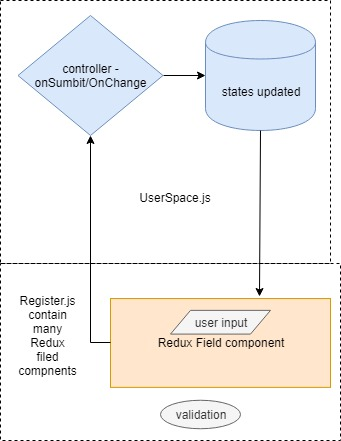
\includegraphics[width=0.5\textwidth]{images/register.jpg}
	\caption{register package process, component diagram}
	\label{fig:}
\end{figure}


The component ResgiterPackage is an assembly of Redux <Field> component and React input.
for each input field the user enter, the page is rendered and the state is updated
The form contain the following validation:
\begin{itemize}
\item No text input filed can be left empty 
\item Receiver mail must be a register user
\end{itemize}
i.e without standing in the form requirement, the user can not press the submit button.

When registering a package, a sensor data may be provided by clicking the correspond checkbox. It is import to mention that not every package has a sensors data.\\*
Algorithm:
\begin{enumerate}
  \item \textbf{http://localhost:8000/address} post request,enter the address and get back and ID for each address provided
    \begin{enumerate}
        \item \textbf {http://localhost:8000/packages}  post request, enter the packages to the packages tables, return a package ID - address ID should be provided
        \begin{enumerate}
        \item \textbf {http://localhost:8000/OrderSensors}  post request, enter the sensors (if exist)  to the sensors table, return a sensor ID - package ID should be provided
        \end{enumerate}
    \item \textbf {http://localhost:8000/OrderHistory}  post request, enter the action(registration) as part of the order history for later on use in the time-line -  package and sensor id should be provided\\
    \end{enumerate}
\end{enumerate}

Only after fetching the data to the database occurred successfully the page content will be replace to a "package have being registered" message.


\subsubsection{Cancel package}
\textbf{http://localhost:3000/\#/packages/active}\\

The feature cancel package allows the user to cancel a package.
After pressing the navbar "delete package" option, the user will be directed to the Activs.js compnent.\newline
The user will be shown a data-minimize table only with packages in a "register" status, \textbf{any other package which has being dispatch already can not be cancel}.\newline
From the system perspective while the package is being canceled, the data is not deleted from storage,it will only be marked as canceled.\\*
Algorithm:
\begin{enumerate}
  \item \textbf{http://localhost:8000/packages/user/}  get request, before component mount: upload all packages with "register" status
  \item If user press delete:
  \begin{enumerate}
      \item \textbf {http://localhost:8000/packages/:id}  put request. Change the spesific package to "cancel" mode.
      \item \textbf {http://localhost:8000/OrderHistory}  post reqest. Update the timeline, add the event to history
\end{enumerate}
\end{enumerate}


\subsubsection{Detailed package view}
\textbf{http://localhost:3000/\#/package/ID}\\
\\*
The feature allows the user to view the extensive package information and the package timeline.
After pressing the specific package ID in the home page,the user will be redirected to rout.The ID will be transfer as a prop from the home page to the the Detailed.js component. 
In addition to the package data which was given during the registration time, the table present the current status of the package and the condition of the package.i.e if the user ask a for a sensor the table will present the amount of events where the condition were not full fill.
The sensor data will be only present if the user register sensors to the package.\\*
Algorithm:
\begin{enumerate}
  \item \textbf{http://localhost:8000/packages/details/id}  get request, before component mount: upload package n information. The information will be display as a table
  \item \textbf{http://localhost:8000/packages/orderHistory/id}  get request, before component mount: upload package history.the history will be sent to the Timeline.js component as a prop.
  \begin{enumerate}
      \item Timeline.js use the npm package "react-horizontal-timeline" to display the package timeline.
      the time line present the status of the package the company and postman name which holds the package at the moment.
    \end{enumerate}
\end{enumerate}





\subsection{Company}

Company user in the system will be able to do the following activities:-

\begin{itemize}
\item \textbf{View package pickup request sent by customer to the particular company.}
When customer registers package, package is registered to DC3 database with registered status. Company will see assigned package on the system filtered by status.
\item \textbf{Accept package pickup request from customer my assigning to the postman under the company.}
The registered package is accepted by company by assigning to available postman of the company for pickup from the customer location. Company does this by clicking Assign button which calls assign.js. Company has to enter the email address of postman on the form and click the button. After the package is assigned to particular postman the status of package will be change to Transit in the database. There is Assign Package Sub-menu under User Management for the package assign function
\item \textbf{Upgrade users to postman or another company user of the same company.}
Company can upgrade registered user to postman or to another company user of the same company by entering email address. For the upgrade function to be applied to particular user. The user has to register themselves as customer first. There is sub menu on sidebar under User Management for this function. UpgradeUser.js is used for this functionality.
\item \textbf{View tracking history of packages under the company.}
When company user login to the system, in the dashboard there will be all the list of packages that have been under the particular company. By clicking on order ID on the leftmost side it takes to detail page of particular company with tracking history of the packages shown as timeline.
\item \textbf{View user list of own company and change their role to available roles in the system.}
Company can see user list of and upgrade individual to postman or another company user as discussed above.
\item \textbf{Create incident for the packages}
Company can create incident for the particular packages if any alteration on the condition is noticed. For this purpose a separate menu is established on sidebar as Incident Management. Incident are created by putting Package ID and incident description under Create Incident sub-menu. 
\item \textbf{View and resolve the incident of particular packages.}
Company can view and resolve the incident for packages if those incident has been resolved. For this company has to click resolve incident button on the incident list displayed in Incidents sub-menu under Incident Management menu.
\end{itemize}


\subsection{Postman}
\textbf{Overview of the functionality:}

Postman user in the system will be able to do the following activities:-
\begin{itemize}
\item {\textbf{View all the packages that have been assigned to him: }}(PostmanTableWithLinks.js) When the Company user assigns a package (PackageId) to a particular postman (PostmanId) then a relevant record is created into the table orderHistory. All the packages that are assigned to the current user are fetched using http://localhost:8000/orderHistory

\item \textbf{View the information about the package such as pickup address, drop address, status etc:} The table orderHistory contains columns that hold the relevant data of the package required for the postman to identify every package.
\item \textbf{Able to change the status of the package as Delivered once the actual delivery has been made:} whenever a postman physically delivers the package to the recipient at the respective Drop Address, then he is able to press the button 'Deliver' that invokes the function to setthe status of the Package as 'Delivered' and enter a new row in the packageHistory table only to denote that the package is now counted as one of the delivered packages.
\item \textbf{Able to Handover the package by assigning it to another Postman and change the status accordingly: }whenever a postman reaches an intermediate point in the route of the package where he has to hand it over to another postman, then the 'Handover' button is used to redirect to another component HandoverForm.js where the user id of the receiving postman needs to be entered. This functionality allows one postman to assign a package to nother postman by changing the 'AssignedTo' data in the relevant table. After this subroutine is invoked the handed over parcel  starts to appear in the dashboard of the receiving postman.
\item \textbf{Able to raise Incident whenever there is any violation of policies:} A postman to who the package has been assigned or handed over is able to judge the condition of the package and raise an incident mentioning the details of the package and the nature of violation also mentioning its current condition using the form created in the Incident.js component.
\item \textbf{View the Incidents that have been raised in the past: }Under the heading 'Incident Management' there is a link 'View Incidents' that redirects to ViewIncidents.js component that pulls data from the Incidents table and allows the Postman to see the relevant list of Incidents raised by or against him that have not yet been resolved.
\end{itemize}

\begin{figure}[htp]
    \centering
    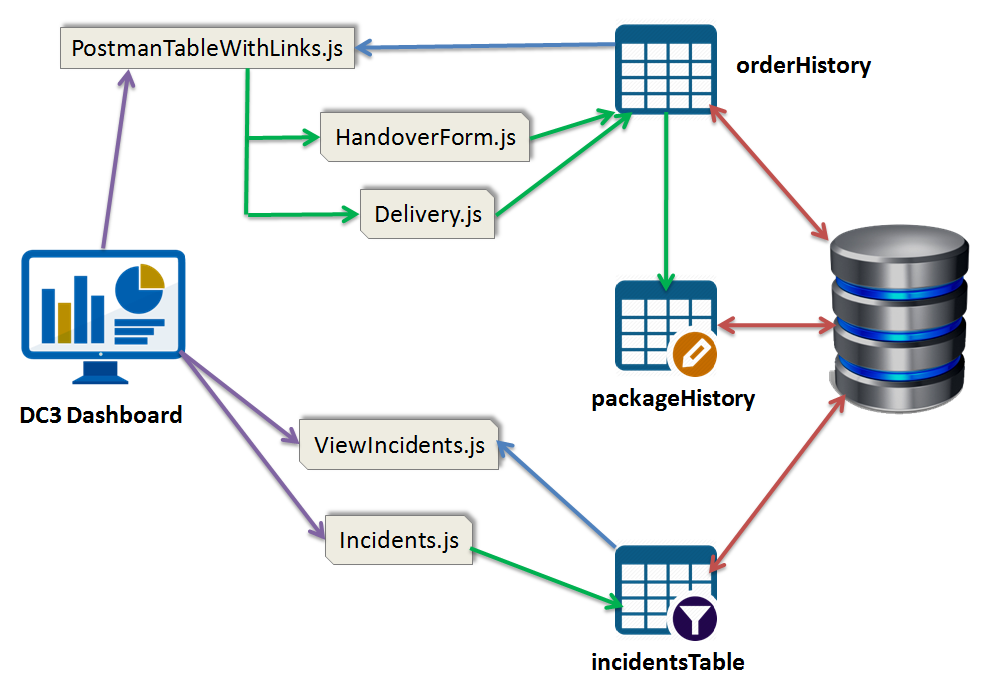
\includegraphics[width=4 cm]{images/snet/DC3 Postman.png}
    \caption{DC3 Postman}
    \label{fig:}
\end{figure}



\section{Back-end}
Back-end or server is a layer on top of the database and Blockchain for the front-end. It does handle the authentication and authorization and does take care of fetching and sending data to the hyper-ledger fabric. We are using following technologies 

\textbf{IDE}: Visual Studio code\\
\textbf{Language}: JavaScript\\
\textbf{Frameworks}: NodeJS with Express



\subsection{Project Structure}
Project structure has is modular and functionality has been divided into folder based on functionality. Hence we have two major folders at the root, server and test, with some other application level files 


\begin{figure}[htp]
    \centering
    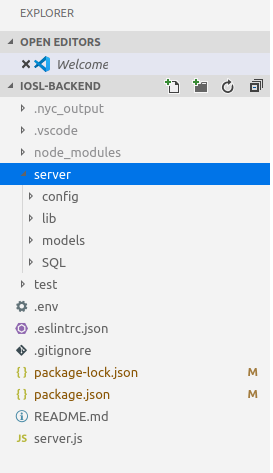
\includegraphics[width=4cm]{images/directystructure.png}
    \caption{Directory Structure}
    \label{fig:}
\end{figure}

\begin{itemize}

\item {\textbf{Server}}: This folder contains all the logic related to server functionality. 
\begin{itemize}
\item {\textbf{Config}}: This folder contains the configuration for the server side. authkeys.js does contain the secret keys used across the application for google social login and to generate the token for authorization. Passport.js contains the logic for google strategy. we can write another strategy in the same file as well e.g. github or local strategy. In future, When we are going to integreate the platform with different vendors, we will be using the local passport strategy using the vendor database. After that, route.js does contain all the routes for the application. any new routes needs to be registered in this file. Finally token.util.js contains utility functions to generate and send the token to the client back. It also exposes the method to generate the token which is used for mocked unit testing. 

\item {\textbf{lib}}: Library or lib folder does contain the middleware for our back-end application. Right now we have only one, secureMiddleware, to secure our API endpoints. It does check if access-token header is provided in rquest body, cookie or querystring and then decode it using our secret. If successful it will set the user profile on the request object, otherwise throw 401 response. 

\item {\textbf{models}}: Models folder does contain all the different models to fetch the data from database or block chain. Each file represent an entity in the system or a related database relation.  Furthermore, index.js file contains the references of all the models and is used almost everywhere in the system as single reference point for the models. 

\item {\textbf{SQL}}: SQL folder contains the database schema which can be used to deploy or create the database while setting up a project on a new machine. Additionally, it contains a schema file to generate the database diagram on dbdiagram.io as well. 
\end{itemize}


\item {\textbf{test}}: This folder contains all the unit tests. Each file contains the tests for the respective model file. Test does use mocha and chai frameworks.

\item {\textbf{env}}: .env is environment file to setup variables at the start of the project instead of reading from the config file, it will be read from the environment. This file is git ignored. It isn't used at the moment as we are reading db config from the db.js directly for now. 

\item {\textbf{eslintrc.json}}: ESlint configuration can be changed using this file. We are using Airbnb base syntax for our linting.  

\item {\textbf{gitignore}}: GitIgnore is used to tell git which files we don't want to store in the source control. 


\item {\textbf{package.json}}: This file contains all the configuration to setup the project. When we do npm install, it will read this file and install all the package on end user machine. It also contains the dev dependencies. We have different scripts configured to run e.g. running the server or run server in the debug mode, run linter. 

\item {\textbf{server.js}}: This is the starting file where our project starts. This file will bootstrap the application by configuring different modules, followed by loading the routes and then running the http server on specific ports. We also configure the express server, body parser (which parse the request body), cookie-parser, passport js and most importantly CORS to send cross origin requests.   

\end{itemize}

\subsection{Unit Testing}
We are using mocha framework for unit and integration testing in our project. Additionally we have used chai as an assertion framework for our tests. Each test has a title or test case description followed by request and expected results. A sample test is as follows

\begin{verbatim}
  /*
  * /GET company/id
  * Test the single company records from the database
  */
  it('It should GET single company', (done) => {
    chai.request(server)
      .get('/company/2')
      .end((err, res) => {
        res.should.have.status(200);
        res.body.should.be.a('array');
        res.body.length.should.be.eql(1);
        done();
      });
  });



\end{verbatim}

We used chai request to call the endpoint, set the access token for the secured endpoints, and then compare the results with  the expectation. We also have tests which will send different access token to validate the authorization of the endpoints e.g. postman can see only packages assigned to him and not all the packages or a customer cannot request a handover for a package. 